\documentclass[11pt,titlepage,twoside]{article}
\usepackage{geometry}                % See geometry.pdf to learn the layout options. There are lots.
\geometry{letterpaper}                   % ... or a4paper or a5paper or ... 
%\geometry{landscape}                % Activate for for rotated page geometry
%\usepackage[parfill]{parskip}    % Activate to begin paragraphs with an empty line rather than an indent
\usepackage{graphicx}
\usepackage{amssymb}
\usepackage{epstopdf}
\usepackage{url}
\usepackage{hyperref}
\usepackage{fancyhdr}
%\DeclareGraphicsRule{.tif}{png}{.png}{`convert #1 `dirname #1`/`basename #1 .tif`.png}

\def\ProgramVersionNoSpace{{VERSION}}
\def\ProgramVersion{{\ProgramVersionNoSpace \space}}
\def\ImagePath{{images}}

\title{Network Extractor \ProgramVersion User Guide}
\author{Cory Quammen}
%\date{}                                           % Activate to display a given date or no date

\usepackage{fancyhdr}
\setlength{\headheight}{15pt}
 
\pagestyle{fancy}
 
\fancyhf{}
\fancyhead[LE,RO]{\thepage}
\fancyhead[RE]{\textit{Network Extractor \ProgramVersion User Guide}}
\fancyhead[LO]{\textit{\nouppercase{\leftmark}}}
 
\fancypagestyle{plain}{ %
\fancyhf{} % remove everything
\renewcommand{\headrulewidth}{0pt} % remove lines as well
\renewcommand{\footrulewidth}{0pt}}

\begin{document}
\maketitle
\tableofcontents
\vfill

\pagebreak

\section{Introduction}

Network Extractor \ProgramVersion is a program for segmenting and collecting statistics on fibrous objects in 3D images. It has been developed with the specific target of fibrin network images in mind, but can be applied to images of any kind of fibrous object such as collagen or actin networks, for example.

Network Extractor \ProgramVersion has been designed in close collaboration with biologists to ensure the most useful features have been implemented. If you have requests for additional features, please contact  \href{mailto:cquammen@cs.unc.edu}{Cory Quammen $\langle$cquammen@cs.unc.edu$\rangle$}.


\subsection{System Requirements}

Network Extractor \ProgramVersion requires Windows XP, Windows 7, or Macintosh OS X 10.5 or higher running on an Intel processor. A recent graphics card is recommended.

Your system should have at least 150 MB of hard drive space free to install the program. At least 512 MB of RAM is required, but 2 GB is recommended.

\subsection{Acknowledgements}

Network Extractor \ProgramVersion is developed and maintained by the \href{http://www.cismm.org}{Center for Computer Integrated Systems for Microscopy and Manipulation}, a \href{http://www.nibib.nih.gov/}{National Institute of Biomedical Imaging and Bioengineering Resource}, award number P41-EB002025.

\section{Installation}

Installation of Network Extractor \ProgramVersion is similar to installation of any other program.

\subsection{Getting the software}

To obtain the latest installer for Network Extractor \ProgramVersionNoSpace, visit \url{http://www.cismm.org/downloads}. Please choose either the Mac or Windows version of the program, whichever is suitable for your system.

Source code for the program is also available there in the form of a Git repository, enabling you full access to the algorithms used to generate the images and providing the opportunity to submit bug fixes back to the project. 

\subsection{Windows installation}

Double-click the setup program named \textbf{Network-Extractor-\ProgramVersionNoSpace-win32.exe}. On the first screen, click \emph{Next}. Please read the program license. If you agree to the terms of the license, click \emph{I Agree}. On the next screen, choose where you want to install the program. The default directory is the most-used option. Click \emph{Next}. You may optionally choose a different location in the Start Menu. By default, it will be placed in the CISMM folder. Click \emph{Install}.

\subsection{Mac installation}

Double-click the Macintosh disk image named \textbf{Network-Extractor-\ProgramVersionNoSpace-darwin.dmg}. An installer program will launch and ask you to agree to the terms of the license. If you agree, a disk image named \textbf{Network-Extractor-\ProgramVersionNoSpace-Darwin} will appear on your desktop and a new Finder window will open.

To install the program in your \emph{Applications} directory on your computer's hard drive, drag the Network Extractor \ProgramVersion application to either the \emph{Applications} alias in the Finder window that just appeared or drag it directly to your \emph{Applications} directory.

\subsection{Running the program}

\subsubsection{Windows}

You can launch the Microscope Simulator program from the Start menu. If you chose the default installation location and menu folder, select \emph{Start} $\rightarrow$ \emph{All Programs} $\rightarrow$ \emph{Network Extractor \ProgramVersionNoSpace} $\rightarrow$ \emph{Network Extractor \ProgramVersionNoSpace}.

\subsubsection{Macintosh}

If you installed the application in the \emph{Applications} directory on your hard drive, double-click the program \emph{Network Extractor \ProgramVersionNoSpace}.

\subsection{Where to get help}

If you have trouble installing or running the program or have questions about its usage, please please contact  \href{mailto:cquammen@cs.unc.edu}{Cory Quammen $\langle$cquammen@cs.unc.edu$\rangle$}. Unfortunately, no guarantee of support can be provided, but we will do our best to help you solve your problem.

\section{Getting to know Network Extractor}

This section gives a tour of the many features in Network Extractor.

\subsection{Program Window}

The program window is shown in Figure \ref{fig:ProgramWindow}. At the top of the window is a standard menu bar. Below the menu bar is the \emph{Visualization Panel} for viewing image data
and segmentation results. Rotating, translating, and scaling the visualization interactively is done by clicking and dragging the mouse within this panel. Four docked windows on the left-hand
side of the window contain control panels for interacting with the program. The \emph{Image Analysis} window contains a control panel for changing settings for the image analysis algorithms. The \emph{Display} window contains controls for changing the visualization of the image data.
The \emph{Tasks} window contains buttons for performing various analysis tasks. Finally, the \emph{Image Information} window  displays information about the image and enables changing of certain settings such as image pixel size. These windows can be undocked from the main 
program window by clicking and dragging in the window's title bar.

\begin{figure}[htbp] %  figure placement: here, top, bottom, or page
   \centering
   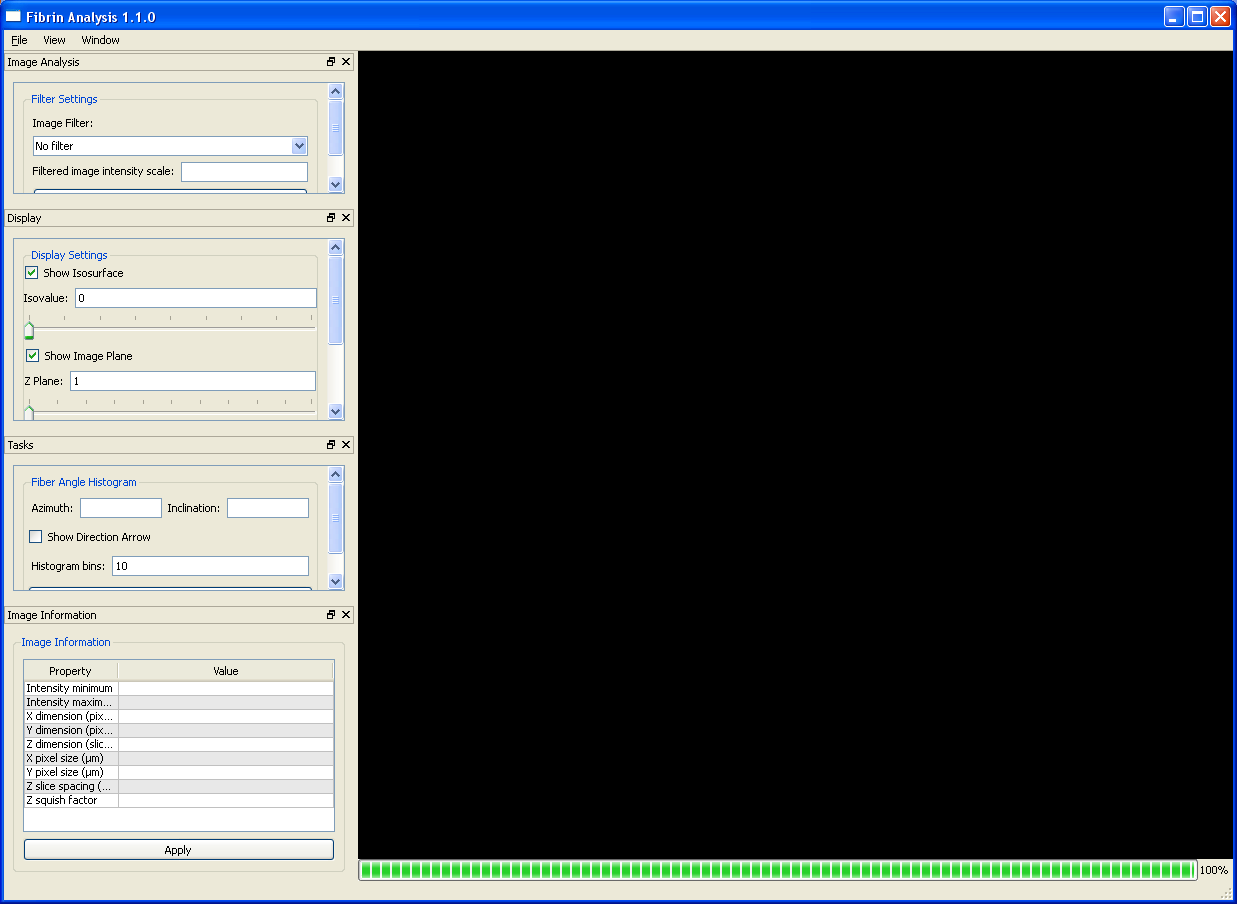
\includegraphics[width=1\linewidth]{\ImagePath/startup_screen} 
   \caption{The program window after startup.}
   \label{fig:ProgramWindow}
\end{figure}

\subsection{Menu Bar}

The menu bar in Network Extractor contains three menus that
provide commands useful for loading data, saving results,
modifying the viewpoint of the visualization, and controlling visibility
of the control panel windows. Each menu is described in more detail below.

\subsubsection{File Menu}

The \emph{File Menu} features commands for loading and saving data:

\begin{description}
  \item[Open Image...] \hfill \\
   Opens an image file. Supported file formats are: multi-layer (3D) TIF, VTK, and LSM. The \href{http://www.loci.wisc.edu/bio-formats/imagej}{LOCI Bio-Formats plug-in}  for \href{http://rsbweb.nih.gov/ij/}{ImageJ} can be used to convert many microscopy file formats into TIF files. Unfortunately, series of TIF images defining a 3D image cannot currently be opened.

  \item[Save Filtered Image...] \hfill \\
  Saves the result of the currently selected image filter in the \emph{Filter Settings} control   panel in the \emph{Image Analysis} window as a 16-bit TIF file.  Use the \emph{Filtered image intensity scale} setting in the \emph{Image Analysis} window to adjust the filtered image intensities to the range [0,65535], the valid range for 16-bit TIF images.

  \item[Save Fiber Orientation Data...] \hfill \\
   Saves a vector image containing the estimated fiber orientation at each voxel in the image. The number of slices ($z$-dimension of the image) may be larger than the input image if the \emph{Z slice spacing} is different from the \emph{X dimension (pixels)} or \emph{Y dimension (pixels)}. In that case, the image will be resampled to produce isotropic voxels. This reduces directional bias in fiber orientation statistics. See Section \ref{sec:CenterlineVoxelsAndOrientationsFile} for details on the file contents.
   
  \item[Open Session...] \hfill \\
  Opens a session file that contains control panel settings. If an image was open when the session file was saved, then this menu item will open that same image.
  
  \item[Save Session...] \hfill \\
  Saves a session file that contains control panel settings.
  
  \item[Save Picture...] \hfill \\
  Saves a screen shot of the visualization panel.
  
  \item[Save Rotation Animation...] \hfill \\
  Saves a series of PNG files containing a rotating animation of the items in the visualization panel.
  
  \item[Save Geometry...] \hfill \\
  Saves a VTK file that contains the geometry of an isosurface from a filtered version of the loaded image. The filter is the one selected in the \emph{Filter Settings} control panel in the \emph{Image Analysis} window. The isovalue is the one  in the \emph{Display Settings} control panel in the \emph{Display} window. 
  
  \item[Exit] \hfill \\
  Exits the program. \textbf{Macintosh users:} The \emph{Quit} menu item appears under the \emph{NetworkExtractor} menu instead of the \emph{File} menu.

\end{description}

%\subsubsection{Edit Menu}
%
%The \emph{Edit Menu} contains functions common to many programs.
%
%\begin{description}
%
%  \item[Cut] \hfill \\
%  \emph{Currently not implemented}
%
%  \item[Copy] \hfill \\
%  \emph{Currently not implemented}
%  
%  \item[Paste] \hfill \\
%  \emph{Currently not implemented}
%
%\end{description}

\subsubsection{View Menu}
\label{sec:ViewMenu}

The \emph{View Menu} has options for saving and loading camera views.

\begin{description}

  \item[Open View...] \hfill \\
  Opens a file specifying camera settings for the visualization panel.
  
  \item[Save View...] \hfill \\
  Saves a file with the current settings of the camera in the visualization panel.

  \item[Reset View] \hfill \\
  Resets the camera so that the image is centered and scaled to fit in the panel and looking towards the bottom z-slice of the image.
  
\end{description}

\subsubsection{Window Menu}

The \emph{Window menu} primarily controls visibility of windows in the program:

\begin{description}

  \item[About Network Extractor] \hfill \\
  Shows a window containing information about Network Extractor. \textbf{Macintosh users:} The \emph{About Network Extractor} menu item appears under the \emph{Network Extractor} menu instead of the \emph{Window} menu. 

  \item[Image Analysis Window] \hfill \\
  Toggle the visibility of the \emph{Image Analysis} window.
  
  \item[Display Window] \hfill \\
  Toggle the visibility of the \emph{Display} window.
  
  \item[Tasks Window] \hfill \\
  Toggle the visibility of the \emph{Tasks} window.
  
  \item[Image Information Window] \hfill \\
  Toggle the visibility of the \emph{Image Information} window.

\end{description}

\subsubsection{Visualization Panel}

Clicking and dragging within the \emph{Visualization Panel} causes manipulation of the camera. You can change the view of the specimen models by rotating, translating, and zooming in
on the scene. Clicking and dragging while holding different mouse buttons enacts these camera transformations:

\begin{itemize}

\item \textbf{Left mouse button} - Rotates the scene

\item \textbf{Middle mouse button} - Translates the scene

\item \textbf{Right mouse button} - Zooms into the scene

\end{itemize}

\subsection{Image Analysis Window}

\begin{figure}[htbp] %  figure placement: here, top, bottom, or page
   \centering
   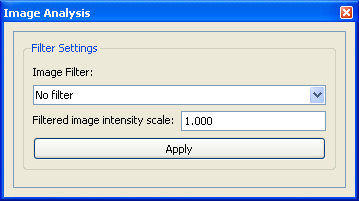
\includegraphics[scale=0.75]{\ImagePath/image_analysis_window} 
   \caption{The \emph{Image analysis} window.}
   \label{fig:ImageAnalysisWindow}
\end{figure}

The \emph{Image Analysis Window} controls which filter is applied to the image. The available filters, explained below, are connected in a pipeline. That is, the result of a filter in the list is fed into the subsequent filter. You can switch between filters to examine results at intermediate steps of the full image analysis pipeline in the visualization panel. The filter results are displayed only as an isosurface; the raw image data is displayed in the image plane. For example, switching to the \emph{Multiscale Fiberness} filter will display the filter results via the isosurface in the
display window. You can then adjust filter parameters based on how well the isosurface
appears to account for fibrous objects in the image.

In addition to determining what the isosurface shows, the selected filter also specifies which data are saved when the \emph{Save Filtered Image...} menu item is chosen in the \emph{File} menu.

Each filter in the \emph{Image Filter} list depends on all of the filters above it. To minimize clutter in the interface, only the settings for the selected filter and those on which it depends are displayed. Each filter and its settings are explained below:

\subsubsection{No filter}
No filter is applied to the image. The raw image data is displayed in the visualization panel.

\begin{description}

\item[Filtered image intensity scale] \hfill \\
This value is a scale factor applied to the output of the selected filter, not just the raw image data. It is typically used to scale the range of the image data to the range [0, 65535], the range of values representable by 16-bit TIF files.

\end{description}

\subsubsection{Multiscale Fiberness}

This filter is based on the paper Frangi, A., Niessen, W., Vincken, K., and Viergever, M.
\href{http://www.springerlink.com/content/a57784628587870p/}{Multiscale vessel enhancement filtering. Medical Image Computing and Computer-Assisted Intervention, 1998, pp. 130--137}. The basic idea is to look at second derivatives of image intensities. For bright fibrous objects on a dark background, the second derivative along the fiber axis has low magnitude while the second derivatives in directions orthogonal to the fiber axis have large negative second derivatives that
are approximately equal. This filter is designed so that voxels satisfying these criteria are assigned a high value and low values are assigned to every other voxel.

This filter searches for fibrous objects of different radii. It does so by taking the second derivative at different scales and keeps only the highest fiberness response from all the scales.

There are several settings for this filter:

\begin{description}

\item[Reject flat objects] \hfill \\
Weighting factor that controls how the filter differentiates fibrous objects from thin, flat objects. Higher values tend to reject flat objects. Setting this value to 0.5 typically works well.

\item[Reject round objects] \hfill \\
Weighting factor that controls how selective the fiberness filter is for fibrous objects versus sphere-like objects. Lower values tend to reject sphere-like objects. Setting this value to 0.5 typically works well.

\item[Reject low contrast objects] \hfill \\
Weighting factor that controls the how much brighter than background objects must be to be identified as fibrous. Higher values of this setting identify highly contrasting fibrous objects. This setting can be important to reduce occurrences of background noise being mis-identified as a
fibrous object. A value of 50.0 typically works well for microscopy images.

\item[Fiber radius minimum ($\mu$m)] \hfill \\
The minimum radius of fibrous objects to be identified by the filter (specified in microns).

\item[Fiber radius maximum ($\mu$m)] \hfill \\
The maximum radius of fibrous objects to be identified by the filter (specified in microns).

\item[Fiber scales] \hfill \\
The number of scales, including the minimum and maximum scales, that will be used to identify fibrous objects. This must be at least 2. The scale space is examined at scale $i$*(fiber radius maximum - fiber radius minimum)/(fiber scales-1) where $i$ is the $i$th scale.

\end{description}

\subsubsection{Multiscale Fiberness Threshold}

This filter creates a binary image (one whose voxel values are restricted to 0 and 1) from the result of the multiscale fiberness filter. All voxels with values above the threshold are set to 1 and all the others are set to 0.

\begin{description}

\item[Fiberness threshold] \hfill \\
The threshold value. One stategy to determine this value is to adjust the isovalue in the \emph{Display Window} so that the isosurface overlaps fibrous objects in the image adequately. Setting the threshold value to this isovalue will ensure that the statistics are taken on all fibrous objects in the image.

\end{description}

\subsubsection{Skeletonization}

\begin{description}

\item[Skeletonization] \hfill \\
Roughly speaking, skeletonization is a process of repeatedly removing voxels from a set of connected voxels until a thin ``curve'' one voxel wide is left. For a fibrous object, the resulting set of voxels, called the \href{http://en.wikipedia.org/wiki/Topological_skeleton}{topological skeleton}, approximates the medial axis of the object. A medial axis is also sometimes called a centerline. There are no settings for this filter.

The algorithm used by this filter is from T.C. Lee, R.L. Kashyap, and C.N. Chu. \href{http://dx.doi.org/10.1006/cgip.1994.1042}{Building skeleton models via 3-D medial surface/axis thinning algorithms. Computer Vision, Graphics, and Image Processing, 56(6):462--478, 1994}. The ITK filter implementation was written by Hanno Homann, Oxford University, Wolfson Medical Vision Lab, UK 
and is available from the \href{http://www.insight-journal.org/browse/publication/181}{Insight Journal}.

\end{description}

\subsection{Display Window}

\begin{figure}[htbp] %  figure placement: here, top, bottom, or page
   \centering
   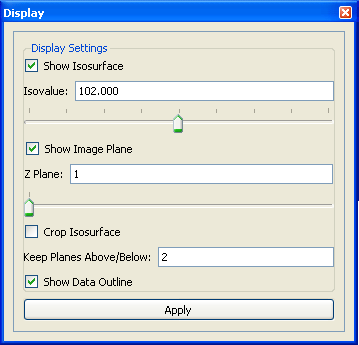
\includegraphics[scale=0.65]{\ImagePath/display_window} 
   \caption{The \emph{Display} window.}
   \label{fig:DisplayWindow}
\end{figure}

The Display Window is where visualization settings can be changed.

\begin{description}

\item[Show isosurface] \hfill \\
Toggles the visibility of the isosurface in the display panel.

\item[Isovalue] \hfill \\
Value that determines the isosurface contour.

\item[Show image plane] \hfill \\
Toggles the visibility of the image plane in the display panel.

\item[Z plane] \hfill \\
Determines which slice of the resampled image with isotropic voxels is displayed in the image plane.

\item[Crop isosurface] \hfill \\
Toggles cropping of the isosurface to a subset of slices centered about the slice displayed in the image plane. Turning this on can be useful for comparing the raw image data to the isosurface showing the filter results.

\item[Keep planes above/below] \hfill \\
Specifies the number of image slices on each side of the image plane through which the isosurface will be taken. The slab of slices defined by this setting is bounded by the extent of the image.

\item[Show data outline] \hfill \\
Toggles the visibility of an outline showing the bounding box of the image.

\end{description}

\subsection{Tasks Window}

\begin{figure}[htbp] %  figure placement: here, top, bottom, or page
   \centering
   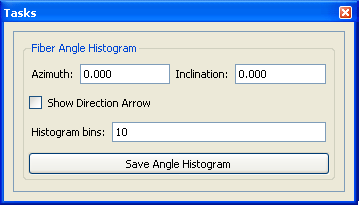
\includegraphics[scale=0.75]{\ImagePath/tasks_window} 
   \caption{The \emph{Tasks} window.}
   \label{fig:TasksWindow}
\end{figure}

This window provides controls for carrying out certain analysis tasks in the program.

The \emph{Fiber Angle Histogram} task saves statistics of the fiber orientations. The histogram
is of angles formed between a reference direction and the orientation of voxel-sized segments along fibers. Orientations of fiber segments are specified by 3D vectors. The program considers vectors $v$ and $-v$ to have equivalent orientations. All orientation vectors are processed so that they point in a set of directions defining a hemisphere. The hemisphere is defined by the plane orthogonal to the reference direction. The re-orientation process ensures that angles between a fiber segment and the reference direction are in the range [0, 90] degrees.

The reference direction is specified by the \emph{Azimuth} and \emph{Inclination}, defined below.

\begin{description}

\item[Azimuth] \hfill \\
The azimuth, specified in degrees, controls the spin angle about the $z$-axis. A setting of 0 degrees, aligns the reference direction with the $x$-axis. That is, when you select the \emph{View}$\rightarrow$\emph{Reset View} option, the arrow will point to the right on the screen when this
setting is 0. A setting of 90 degrees will point the reference direction up on the screen.

\item[Inclination] \hfill \\
The inclination, also specified in degrees, controls the angle between the reference direction and the $xy$-plane. If you select the \emph{View}$\rightarrow$\emph{Reset View} option, this setting moves the tip of the reference direction above or below the screen plane. A positive value lifts the tip up in the $z$-direction (toward you) while a negative value pushes it down (away from you).

\item[Show direction arrow] \hfill \\
Toggle the visibility of an arrow showing the reference direction.

\item[Histogram bins] \hfill \\
Controls the number of bins in the angle histogram.

\end{description}

The angle histogram can be saved by clicking the \emph{Save angle histogram} button. See
Section \ref{sec:FiberAngleHistogramFileSection} below for details of the file contents.

\subsection{Image Information Window}

\begin{figure}[htbp] %  figure placement: here, top, bottom, or page
   \centering
   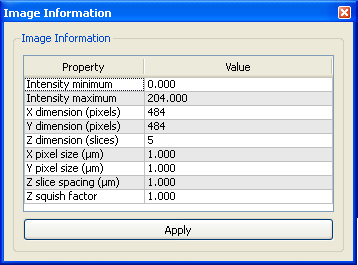
\includegraphics[scale=0.75]{\ImagePath/image_information_window} 
   \caption{The \emph{Image information} window.}
   \label{fig:ImageInformationWindow}
\end{figure}

The Image Information Window displays information about the image loaded into the program. The last four settings are editable while the others are not.

\begin{description}

\item[Intensity minimum] \hfill \\
Minimum intensity value in the filtered image.

\item[Intensity maximum] \hfill \\
Maximum intensity value in the filtered image.

\item[X dimension (pixels)] \hfill \\
Dimension of image in the $x$-direction (how many pixels).

\item[Y dimension (pixels)] \hfill \\ 
Dimension of image in the $y$-direction (how many pixels).

\item[Z dimension (slices)] \hfill \\
Dimension of image in the $z$-direction (how many slices).

\item[X pixel size ($\mu$m)] \hfill \\ 
The size of the pixel, or spacing between pixels, in the $x$-direction (voxel x-spacing). \emph{Editable}.

\item[Y pixel size ($\mu$m)] \hfill \\
The size of the pixel, or spacing between pixels, in the $y$-direction (voxel y-spacing). \emph{Editable}.

\item[Z slice spacing ($\mu$m)] \hfill \\
The spacing between slices in the image (voxel $z$-spacing). \emph{Editable}.

\item[Z squish factor] \hfill \\
This value specifies a scale factor for the $z$-spacing of the image that is not the same as the Z slice spacing. The squish factor is meant as a way to correct for the apparent elongation of objects in the $z$-direction in images from confocal microscopes. This elongation is an artifact caused by the point-spread function of the microscope. Setting the Z squish factor to a value below 1.0 will compress the image in the $z$-dimension, essentially undoing the elongation caused by the point-spread function. For confocal microscopes, a Z squish factor of 0.5 works well. \emph{Editable}.

\end{description}

The \emph{Apply} button will apply the editable settings as well as any setting changes in the \emph{Image Analysis} and \emph{Display} windows.

\section{Output Files}
\label{sec:CenterlineVoxelsAndOrientationsFile}

Network Extractor writes two kinds of files for reporting information about orientations of fibrous objects in images. There are two types of files:

\begin{description}

\item[Centerline voxels and orientations file]

This file is produced when the \emph{File}$\rightarrow$\emph{Save Fiber Orientation Data...}
menu item is selected. To export this file, the \emph{Skeletonization} filter in the \emph{Image Analysis} window must be applied.

This file is a comma-separated file that can be imported into popular spreadsheet programs. The file has six columns:

\begin{itemize}

  \item \textbf{xPosition}  - The $x$-coordinate of the fiber voxel.
  
  \item \textbf{yPosition} - The $y$-coordinate of the fiber voxel.
  
  \item \textbf{zPosition} - The $z$-coordinate of the fiber voxel.
  
  \item \textbf{xDirection} - The $x$-component of the fiber orientation vector.
  
  \item \textbf{yDirection} - The $y$-component of the fiber orientation vector.
  
  \item \textbf{zDirection} - The $z$-component of the fiber orientation vector.

\end{itemize}

\item[Fiber angle histogram file] \hfill \\
\label{sec:FiberAngleHistogramFileSection}
This file is produced when the \emph{Save angle histogram} button is clicked in the \emph{Tasks Window}.

This file is a comma-separated file that can be imported into popular spreadsheet programs. The file has six columns:

\begin{itemize}

  \item \textbf{Angle (deg.)} - The minimum value in the histogram bin. The maximum value in the histogram bin is given by the next row in this column. The maximum angle on the last bin is 90 degrees.
  
  \item \textbf{Count} - The number of image voxels in the histogram bin.
  
  \item \textbf{Normalized Count} - The number of image voxels in the histogram bin divided by the total number of voxel values in the histogram.

  \item \textbf{Expected Probability} - The expected normalized histogram value for an object with uniform randomly distributed orientation of fiber segments.
  
  \item \textbf{Over-representation Ratio} - The normalized count divided by the expected probability. This gives an indication of whether and to what degree the orientations within a histogram bin are overrepresented. A value of 1.0 means the number of orientations of fiber segments falling into this bin is expected, a value below 1.0 means there are fewer fiber segments falling in this bin than expected, and a value above 1.0 means there are more fiber segments falling into the bin than expected for an object with uniform randomly distributed orientations.

\end{itemize}

\end{description}

%\pagebreak

\section{Version History}

\subsection{Version 1.0.0}

%\noindent
%Changes from previous release:
%\begin{itemize}
%\item Complete rewrite of the Microscope Simulator program.
%\end{itemize}

Initial release.

\noindent
Known issues:
\begin{itemize}

\item None

\end{itemize}

\end{document}  